\documentclass{article}

\def\npart{III}
\def\nyear{2018}
\def\nterm{Michaelmas}
\def\nlecturer{Dr. S. Barbina}
\def\ncourse{Model Theory}
\def\draft{Ongoing course, rough}
\usepackage{mathrsfs}
\usepackage{imakeidx}
\usepackage{marginnote}
\ifx \nauthor\undefined
  \def\nauthor{Bhavik Mehta}
\else
\fi

\author{Based on lectures by \nlecturer \\\small Notes taken by \nauthor}
\date{\nterm\ \nyear}
\title{Part \npart\ -- \ncourse}

\usepackage[utf8]{inputenc}
\usepackage{amsmath}
\usepackage{amsthm}
\usepackage{amssymb}
\usepackage{enumerate}
\usepackage{mathtools}
\usepackage{graphicx}
\usepackage[dvipsnames]{xcolor}
\usepackage{tikz}
\usepackage{wrapfig}
\usepackage{centernot}
\usepackage{float}
\usepackage{braket}
\usepackage[hypcap=true]{caption}
\usepackage{enumitem}
\usepackage[colorlinks=true, linkcolor=mblue]{hyperref}
\usepackage[nameinlink,noabbrev]{cleveref}
\usepackage{nameref}
\usepackage[margin=1.5in]{geometry}

% Theorems
\theoremstyle{definition}
\newtheorem*{aim}{Aim}
\newtheorem*{axiom}{Axiom}
\newtheorem*{claim}{Claim}
\newtheorem*{cor}{Corollary}
\newtheorem*{conjecture}{Conjecture}
\newtheorem*{defi}{Definition}
\newtheorem*{eg}{Example}
\newtheorem*{ex}{Exercise}
\newtheorem*{fact}{Fact}
\newtheorem*{law}{Law}
\newtheorem*{lemma}{Lemma}
\newtheorem*{notation}{Notation}
\newtheorem*{prop}{Proposition}
\newtheorem*{question}{Question}
\newtheorem*{rrule}{Rule}
\newtheorem*{thm}{Theorem}
\newtheorem*{assumption}{Assumption}

\newtheorem*{remark}{Remark}
\newtheorem*{warning}{Warning}
\newtheorem*{exercise}{Exercise}

% \newcommand{\nthmautorefname}{Theorem}

\newtheorem{nthm}{Theorem}[section]
\newtheorem{nlemma}[nthm]{Lemma}
\newtheorem{nprop}[nthm]{Proposition}
\newtheorem{ncor}[nthm]{Corollary}
\newtheorem{ndef}[nthm]{Definition}

% Special sets
\newcommand{\C}{\mathbb{C}}
\newcommand{\N}{\mathbb{N}}
\newcommand{\Q}{\mathbb{Q}}
\newcommand{\R}{\mathbb{R}}
\newcommand{\Z}{\mathbb{Z}}

\newcommand{\abs}[1]{\left\lvert #1\right\rvert}
\newcommand{\norm}[1]{\left\lVert #1\right\rVert}
\renewcommand{\vec}[1]{\boldsymbol{\mathbf{#1}}}

\let\Im\relax
\let\Re\relax

\DeclareMathOperator{\Im}{Im}
\DeclareMathOperator{\Re}{Re}
\DeclareMathOperator{\id}{id}

\definecolor{mblue}{rgb}{0., 0.05, 0.6}

\makeindex[intoc]

% preamble

\reversemarginpar

\let\oldmodels\models
\let\models\vDash
\let\nModels\nvDash

\setcounter{section}{-1}

\DeclareMathOperator{\Mod}{Mod}
\DeclareMathOperator{\Th}{Th}
\DeclareMathOperator{\dom}{dom}
\DeclareMathOperator{\img}{img}
\DeclarePairedDelimiter\ceil{\lceil}{\rceil}
\DeclarePairedDelimiter\floor{\lfloor}{\rfloor}

\newtheorem{nremark}[nthm]{Remark}
\newtheorem{nexample}[nthm]{Example}
\newtheorem{nexercise}[nthm]{Exercise}
\newtheorem{nfact}[nthm]{Fact}
\newtheorem{nnotation}[nthm]{Notation}

\newcommand{\named}[1]{\textbf{#1}\index{#1}}

%\newtheorem{manualtheoreminner}{Theorem}
%\newenvironment{manualtheorem}[1]{%
%    \renewcommand\themanualtheoreminner{#1}%
%    \manualtheoreminner
%}{\endmanualtheoreminner}

% and here we go!

\begin{document}
\maketitle

\tableofcontents

\clearpage
\marginnote{\emph{Lecture 1}}[0cm]
\section{Introduction}
Model theory is a part of logic that began by looking at algebraic objects such as groups and combinatorial objects such like graphs, described in formal language.
The basic question in model theory is: `how powerful is our description of these objects to pin them down'?
In Logic and Set Theory, the focus was on what was provable from a theory and language, but here we focus on whether or not a model exists.

\section{Languages and structures}
\begin{ndef}[Language]\label{def:1.1}\hypertarget{def:lang}
  A \named{language} $L$ consists of
  \begin{enumerate}[label=(\roman*)]
    \item a set $\mathscr{F}$ of function symbols, and for each $f \in \mathscr{F}$ a positive integer $m_f$ the \named{arity} of $f$.
    \item a set $\mathscr{R}$ of relation symbols, and for each $R \in \mathscr{R}$, a positive integer $m_R$.
    \item a set $\mathscr{C}$ of constant symbols.
  \end{enumerate}
  Note: each of $\mathscr{F}, \mathscr{R}$ and $\mathscr{C}$ can be empty.
\end{ndef}
\begin{eg}
  \hypertarget{def:lgp}Take $L = \{\{\cdot , ^{-1}\}, \{1\}\}$, for $\cdot$ a binary function and $^{-1}$ an unary function, $1$ a constant. This is the \hyperlink{def:lang}{language} of groups, call it $L_{\text{gp}}$.
  Also, $L_{\text{lo}} = \{<\}$ a single binary relation, for linear orders.
\end{eg}

\begin{ndef}[$L$-structure]\label{def:1.2}\index{structure}\hypertarget{def:lstr}
  Given a \hyperlink{def:lang}{language} $L$, say, an \textbf{$L$-structure} consists of
  \begin{enumerate}[label=(\roman*)]
    \item a set $M$, the \named{domain}
    \item for each $f \in \mathscr{F}$, a function $f^\mathcal{M} : M^{m_f} \to M$.
    \item for each $R \in \mathscr{R}$, a relation $R^\mathcal{M} \subseteq M^{m_R}$.
    \item for each $c \in \mathscr{C}$, an element $c^\mathcal{M} \in M$.
  \end{enumerate}
  $f^M, R^M, c^M$ are the \named{interpretations} of $f,R,c$ respectively.
\end{ndef}
\begin{nremark}\label{rem:1.3}
  We often fail to distinguish between the \hyperlink{def:lang}{symbols} in $L$ and their \hyperlink{def:lstr}{interpretations} in a \hyperlink{def:lstr}{structure}, if the interpretations are clear from the context.
\end{nremark}

We may write $\mathcal{M} = \langle M, \mathscr{F}, \mathscr{R}, \mathscr{C} \rangle$.

\begin{nexample}\label{eg:1.4}\leavevmode
  \begin{enumerate}[label=(\alph*)]
    \item $\mathcal{R} = \langle \mathbb{R}^+, \{\cdot, ^{-1}\}, 1 \rangle$ is an \hyperlink{def:lgp}{$L_{\text{gp}}$}-\hyperlink{def:lstr}{structure}.
    \item $\mathcal{Z} = \langle \mathbb{Z}, \{+, -\}, 0 \rangle$ is an $L_{\text{gp}}$-structure.
    \item $\mathcal{Q} = \langle \mathbb{Q}, < \rangle$ is an \hyperlink{def:lgp}{$L_{\text{lo}}$}-structure.
  \end{enumerate}
\end{nexample}
\begin{ndef}[Embedding]\label{def:1.5}\hypertarget{def:embedding}
  Let $L$ be a \hyperlink{def:lang}{language}, let $\mathcal{M}, \mathcal{N}$ be \hyperlink{def:lstr}{$L$-structures}.
  An \named{embedding} of $\mathcal{M}$ into $\mathcal{N}$ is a one-to-one mapping $\alpha: M \to N$ such that
  \begin{enumerate}[label=(\roman*)]
    \item for all $f \in \mathscr{F}$, and $a_1, \dotsc, a_{m_f} \in M$,
      \begin{equation*}
        \alpha(f^\mathcal{M}(a_1, \dotsc, a_{n_f})) = f^\mathcal{N}(\alpha(a_1), \dotsc, \alpha(a_{n_f}))
      \end{equation*}
      \begin{center}
        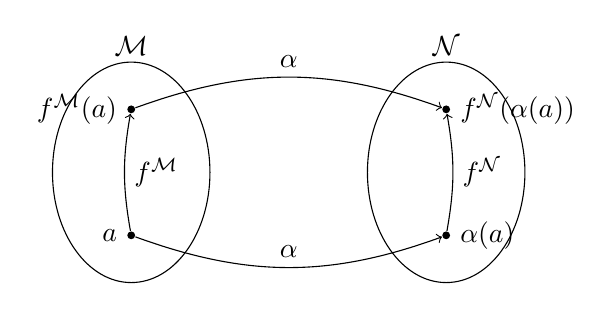
\begin{tikzpicture}[scale=1]
          \node at (-2, 1.6) {$\mathcal{M}$};
          \node at (2, 1.6) {$\mathcal{N}$};
          \draw (-2, 0) circle [x radius=10mm, y radius=14mm];
          \node [circle, inner sep=1pt, fill=black, label=left:$a$] (a) at (-2, -0.8) {};
          \node [circle, inner sep=1pt, fill=black, label=left:$f^\mathcal{M}(a)$] (fa) at (-2, 0.8) {};
          \draw (2, 0) circle [x radius=10mm, y radius=14mm];
          \node [circle, inner sep=1pt, fill=black, label=right:$\alpha(a)$] (aa) at (2, -0.8) {};
          \node [circle, inner sep=1pt, fill=black, label=right:$f^\mathcal{N}(\alpha(a))$] (faa) at (2, 0.8) {};
          \draw [->] (a) to [bend right=20] node[above]{$\alpha$} (aa);
          \draw [->] (fa) to [bend left=20] node[above]{$\alpha$} (faa);
          \draw [->] (a) to [bend left=10] node[right]{$f^\mathcal{M}$} (fa);
          \draw [->] (aa) to [bend right=10] node[right]{$f^\mathcal{N}$} (faa);
        \end{tikzpicture}
      \end{center}
    \item for all $R \in \mathscr{R}$, and $a_1, \dotsc, a_{n_R} \in M$
      \begin{equation*}
        (a_1, \dotsc, a_{n_R}) \in R^\mathcal{M} \iff (\alpha(a_1), \dotsc, \alpha(a_{n_R})) \in R^\mathcal{N}
      \end{equation*}
    \item for all $c \in \mathscr{C}$, $\alpha(c^\mathcal{M}) = c^\mathcal{N}$.
  \end{enumerate}
  \hypertarget{def:iso}An \named{isomorphism} of $\mathcal{M}$ into $\mathcal{N}$ is a surjective embedding (onto).
\end{ndef}

\begin{nexercise}\label{ex:1.6}
  Let $G_1, G_2$ be groups, regarded as \hyperlink{def:lgp}{$L_{\text{gp}}$}-structures.
  Check that $G_1 \simeq G_2$ in the usual algebra sense if and only if there is an \hyperlink{def:iso}{isomorphism} $\alpha: G_1 \to G_2$ in the sense of \cref{def:1.5}.
\end{nexercise}

\clearpage
\section{Review: Terms, formulae and their interpretations}
In addition to the \hyperlink{def:lang}{symbols} of $L$, we also have
\begin{enumerate}[label=(\roman*)]
  \item infinitely many variables $\{x_i\}_{i \in I}$
  \item logical connectives $\wedge, \neg$ (also expresses $\vee, \implies, \iff$)
    \item quantifier $\exists$ (also expresses $\forall$)
    \item $(\phantom{-},\phantom{-})$
    \item equality symbol $=$
\end{enumerate}

\begin{ndef}[\hypertarget{def:lterm}{$L$-terms}]\label{def:2.1}
  \index{term}\textbf{$L$-terms} are defined recursively as follows:
  \begin{itemize}[label=--]
    \item any variable $x_i$ is a term
    \item any constant symbol is a term
    \item for any $f \in \mathscr{F}$, $f(t_1, \dotsc, t_{m_f})$ for any terms $t_1, \dotsc, t_{m_f}$ is a term
    \item nothing else is a term
  \end{itemize}
\end{ndef}

Notation: we write $t(x_1, \dotsc, x_m)$ to mean that the variables appearing in $t$ are among $x_1, \dotsc, x_m$.
\begin{eg}
  \marginnote{\emph{Lecture 2}}[0cm]
  Take $\mathcal{R} = \langle \mathbb{R}^*, \{\cdot, ^{-1}\}, 1 \rangle$.
  Then $\cdot ( \cdot(x_1, x_2), x_3)$ is a \hyperlink{def:lterm}{term}, usually written $(x_1 \cdot x_2) \cdot x_3$.
  Also, $(\cdot (1, x_1))^{-1}$ is a \hyperlink{def:lterm}{term}, written $(1\cdot x)^{-1}$
\end{eg}
\begin{ndef}\label{def:2.2}
  If $\mathcal{M}$ is an \hyperlink{def:lstr}{$L$-structure}, to each \hyperlink{def:lterm}{$L$-term} $t(x_1, \dotsc, x_k)$ we assign a function
  a function $t^\mathcal{M}: M^k \to M$ defined as follows:
  \begin{enumerate}[label=(\roman*)]
    \item If $t = x_i$, $t^\mathcal{M}[a_1, \dotsc, a_k] = a_i$
    \item If $t = c$, $t^\mathcal{M}[a_1, \dotsc, a_k] = c^\mathcal{M}$.
    \item If $t = f(t(x_1, \dotsc, x_k), \dotsc, t_{m_f}(x_1, \dotsc, x_k))$,
      \begin{equation*}
        t^\mathcal{M}(a_1, \dotsc, a_k) = f^\mathcal{M}(t_1^\mathcal{M}(a_1, \dotsc, a_k), \dotsc, t^\mathcal{M}_{m_f}(a_1, \dotsc, a_k))
      \end{equation*}
  \end{enumerate}
\end{ndef}

Notice in $L_{\text{gp}}$, the term $x_2 \cdot x_3$ can be described as $t_1(x_1, x_2, x_3)$ or $t_2(x_1, x_2, x_3, x_4)$, or infinitely many other ways.
Then $t_1$ is assigned to $t_1^\mathcal{M}: M^3 \to M$, with $(a_1, a_2, a_3) \mapsto (a_2, a_3)$, and $t_2$ is assigned to $t_2^\mathcal{M} : M^4 \to M$, with $(a_1, a_2, a_3, a_4) \mapsto a_2 \cdot a_3$.
\begin{nfact}\label{fact:2.3}
  Let $\mathcal{M}, \mathcal{N}$ be \hyperlink{def:lstr}{$L$-structures}, and let $\alpha: \mathcal{M} \to \mathcal{N}$ be an \hyperlink{def:embedding}{embedding}.
  For any \hyperlink{def:lterm}{$L$-term} $t(x_1, \dotsc, x_k)$ and $a_1, \dotsc, a_k \in M$ we have
  \begin{equation*}
    \alpha(t^\mathcal{M}(a_1, \dotsc, a_k)) = t^\mathcal{N}(\alpha(a_1), \dotsc, \alpha(a_k))
  \end{equation*}
\end{nfact}
\begin{proof}
  By induction on the complexity of $t$. Let $\bar{a} = (a_1, \dotsc, a_k)$ and $\bar{x} = (x_1, \dotsc, x_k)$.
  Then
  \begin{enumerate}[label=(\roman*)]
    \item if $t = x_i$, then $t^\mathcal{M}(\bar{a}) = a_i$, and $t^\mathcal{N}(\alpha(a_1), \dotsc, \alpha(a_k)) = \alpha(a_i)$, so the conclusion holds.
    \item if $t = c$ a constant, then $t^\mathcal{M}(\bar{a}) = c^\mathcal{M}$, and $t^\mathcal{N}(\alpha(\bar{a})) = c^\mathcal{N}$, and $\alpha(c^\mathcal{M}) = c^\mathcal{N}$, as required.
    \item if $t = f(t_1(\bar{x}),\dotsc, t_{m_f}(\bar{x}))$, then
      \begin{equation*}
        \alpha(f^\mathcal{M}(t_1^\mathcal{M}(\bar{a}), \dotsc, t_{m_f}^\mathcal{M}(\bar{a}))) = f^\mathcal{N}(\alpha(t_1^\mathcal{M}(\bar{a})), \dotsc, \alpha(t_{m_f}^\mathcal{M}(\bar{a})))
      \end{equation*}
      since $\alpha$ is an \hyperlink{def:embedding}{embedding}.
      $t_1(\bar{x}), \dotsc, t_{m_f}(\bar{x})$ have lower complexity than $t$, so inductive hypothesis applies. \qedhere
  \end{enumerate}
\end{proof}
\begin{nexercise}\label{ex:2.4}
  Exercise: conclude the proof of \cref{fact:2.3}.
\end{nexercise}
\begin{ndef}[Atomic formula]\label{def:2.5}\index{formula!atomic}\hypertarget{def:atomform}
  The set of \named{atomic formulas} of $L$ is defined as follows
  \begin{enumerate}[label=(\roman*)]
    \item if $t_1, t_2$ are $L$-terms, then $t_1 = t_2$ is an atomic formula
    \item if $R$ is a relation symbol and $t_1, \dotsc, t_{m_R}$ are terms, then $R(t_1, \dotsc, t_{m_R})$ is an atomic formula
    \item nothing else is an atomic formula.
  \end{enumerate}
\end{ndef}
\begin{ndef}[Formula]\label{def:2.6}\index{formula}\hypertarget{def:form}
  The set of \textbf{$L$-formulas} is defined as follows
  \begin{enumerate}[label=(\roman*)]
    \item any \hyperlink{def:atomform}{atomic formula} is an $L$-formula
    \item if $\phi$ is an $L$-formula, then so is $\neg \phi$
    \item if $\phi$ and $\psi$ are $L$-formulas, then so is $\phi \wedge \psi$
    \item if $\phi$ is an $L$-formula, for any $i \geq 1$, $\exists x_i \; \phi$ is an $L$-formula
    \item nothing else is an $L$-formula
  \end{enumerate}
\end{ndef}
\begin{eg}
  In $L_{\text{gp}}$, $x_1 \cdot x_1 = x_2$ and $x_1 \cdot x_2 = 1$ are \hyperlink{def:form}{atomic formulas}, and $\exists x_1 \; (x_1 \cdot x_2) = 1$ is an $L_{\text{gp}}$-formula.
\end{eg}
\hypertarget{def:free}A variable occurs freely in a formula if it does not occur within the scope of a quantifier $\exists$ (the variable is \named{free}). Otherwise the variable is \named{bound}. For instance, in $\exists x_1 \; (x_1 \cdot x_2) = 1$, $x_1$ is bound and $x_2$ is free.

\textbf{Important convention:} no variable occurs both \hyperlink{def:free}{freely} and as a bound variable in the same formula.

\hypertarget{def:sentence}A \named{sentence} is a \hyperlink{def:form}{formula} with no \hyperlink{def:free}{free} variables. $\exists x_1 \exists x_2 \; (x_1 \cdot x_2 = 1)$ is an $L_{\text{gp}}$-sentence.
Notation: $\phi(x_1, \dotsc, x_k)$ means that the free variables in $\phi$ are among $x_1, \dotsc, x_k$.

\begin{ndef}[$\models$]\label{def:2.7}\index{$\models$}\hypertarget{def:models}
  Let $\phi(x_1, \dotsc, x_k)$ be an \hyperlink{def:form}{$L$-formula}, let $\mathcal{M}$ be an \hyperlink{def:lstr}{$L$-structure}, and let $\bar{a} = (a_1, \dotsc, a_k)$ be elements of $M$.
  We define $\mathcal{M} \models \phi(\bar{a})$ as follows.
  \begin{enumerate}[label=(\roman*)]
    \item if $\phi$ is $t_1 = t_2$, then $\mathcal{M} \models \phi(\bar{a})$ if and only if $t_1^\mathcal{M}(\bar{a}) = t_2^\mathcal{M}(\bar{a})$.
    \item if $\phi$ is $R(t_1, \dotsc, t_{m_k})$ then $\mathcal{M} \models \phi(\bar{a})$ iff
      \begin{equation*}
        (t_1^\mathcal{M}(\bar{a}),\dotsc,t_{m_k}^\mathcal{M}(\bar{a})) \in R^\mathcal{M}.
      \end{equation*}
    \item if $\phi$ is $\psi \wedge \chi$, then $\mathcal{M} \models \phi(\bar{a})$ iff $\mathcal{M} \models \psi(\bar{a})$ and $\mathcal{M} \models \chi(\bar{a})$.
    \item if $\phi = \neg \psi$ then $\mathcal{M} \models \phi(\bar{a})$ iff $\mathcal{M} \nModels \psi(\bar{a})$. (this is well-defined since $\psi(\bar{a})$ is shorter than $\phi(\bar{a})$)
    \item if $\phi$ is $\exists x_j: \chi(x_1, \dotsc, x_k, x_j)$ (where $x_j \neq x_i$ for $i = 1, \dotsc, k$).
      Then $\mathcal{M} \models \phi(\bar{a})$ iff there is $b \in \mathcal{M}$ such that $\mathcal{M} \models \chi(a_1, \dotsc, a_k, b)$.
  \end{enumerate}
\end{ndef}
\begin{eg}
  For $\mathcal{R} = \langle \mathbb{R}^*,\cdot, ^{-1}, 1\rangle$, if $\phi(x_1) = \exists x_2 \; (x_2 \cdot x_2) = x_1$ then $\mathcal{R} \hyperlink{def:models}{\models} \phi(1)$ but $\mathcal{R} \nModels \phi(-1)$.
\end{eg}
\begin{nnotation}[Useful abbreviations]\label{not:2.8}
  We write
  \begin{itemize}[label=--]
    \item $\phi \vee \psi$ for $\neg(\neg\phi \wedge \neg\psi)$
    \item $\phi \to \psi$ for $\neg \phi \vee \psi$
    \item $\phi \leftrightarrow \psi$ for $(\phi \to \psi) \wedge (\psi \to \phi)$
    \item $\forall x_i\ \phi$ for $\neg \exists x_i\ (\neg \phi)$
  \end{itemize}
\end{nnotation}
\begin{nprop}\label{prop:2.9}
  Let $\mathcal{M}, \mathcal{N}$ be \hyperlink{def:lstr}{$L$-structures}, let $\alpha: \mathcal{M} \to \mathcal{N}$ be an \hyperlink{def:embedding}{embedding}.
  Let $\phi(\bar{x})$ be \hyperlink{def:atomform}{atomic} and $\bar{a} \in M^{|\bar{x}|}$, then
  \begin{equation*}
    M \hyperlink{def:models}{\models} \phi(\bar{a}) \iff \mathcal{N} \models \phi(\alpha(\bar{a})).
  \end{equation*}
\end{nprop}

Question: If $\phi$ is an \hyperlink{def:form}{$L$-formula}, not necessarily \hyperlink{def:atomform}{atomic}, does \cref{prop:2.9} hold?

\marginnote{\emph{Lecture 3}}[0cm]
\begin{proof}[Proof of \cref{prop:2.9}]
  Cases:
  \begin{enumerate}[label=(\roman*)]
    \item $\phi(\bar{x})$ is of the form $t_1(\bar{x}) = t_2(\bar{x})$ where $t_1,t_2$ are terms.
      (Exercise: complete this case, using \cref{fact:2.3})
    \item $\phi(\bar{x})$ is of the form $R(t_1(\bar{x}), \dotsc, t_{m_R}(\bar{x}))$.
      Then $\mathcal{M} \hyperlink{def:models}{\models} R(t_1(\bar{a}), \dotsc, t_{m_R}(\bar{a}))$ if and only if...
      (Exercise: complete this case)
  \end{enumerate}
\end{proof}
\begin{nexercise}\label{ex:2.10}
  Show that \cref{prop:2.9} holds if $\phi(\bar{x})$ is a formula without quantifiers (a quantifier-free formula).
\end{nexercise}
\begin{nexample}\label{ex:2.11}
  Do \hyperlink{def:embedding}{embeddings} preserve \emph{all} \hyperlink{def:form}{formulas}? No.
  Take $\mathcal{Z} = (\mathbb{Z}, <)$ and $\mathcal{Q} = (\mathbb{Q}, <)$ an \hyperlink{def:lgp}{$L_{\text{lo}}$}-\hyperlink{def:lstr}{structure}
  Then $\alpha: \mathbb{Z} \to \mathbb{Q}$ (inclusion) is an embedding, but
  \begin{gather*}
    \phi(x_1, x_2) = \exists x_3\,(x_1 < x_3 \wedge x_3 < x_2). \\
    \mathcal{Q} \hyperlink{def:models}{\models} \phi(1,2) \text{ but } \mathcal{Z} \nModels \phi(1,2).
  \end{gather*}
\end{nexample}
\begin{nfact}\label{fact:2.12}
  Let $\alpha: \mathcal{M} \to \mathcal{N}$ be an \hyperlink{def:iso}{isomorphism}.
  Then if $\phi(\bar{x})$ is an \hyperlink{def:form}{$L$-formula} and $\bar{a} \in M^{|\bar{x}|}$, then
  \begin{equation*}
    \mathcal{M} \hyperlink{def:models}{\models} \phi(\bar{a}) \iff \mathcal{M} \models \phi(\alpha(\bar{a})).
  \end{equation*}
\end{nfact}
\begin{proof}
  Exercise.
\end{proof}

\clearpage
\section{Theories and elementarity}
Throughout, $L$ is a \hyperlink{def:lang}{language}, $\mathcal{M}, \mathcal{N}$ are \hyperlink{def:lstr}{$L$-structures}.
\begin{ndef}[$L$-theory]\label{def:3.1}\index{theory}\hypertarget{def:ltheory}
  An \textbf{$L$-theory} $T$ is a set of \hyperlink{def:sentence}{$L$-sentences}.
  \hypertarget{def:model}$\mathcal{M}$ is a \named{model} of $T$ if $\mathcal{M} \hyperlink{def:models}{\models} \sigma$ for all $\sigma \in T$. We write $\mathcal{M} \models T$.
  The class of all the models of $T$ is written $\Mod(T)$.
  The theory of $\mathcal{M}$ is the set
  \begin{equation*}
    \Th(\mathcal{M}) = \set{\sigma | \sigma \text{ is an } L\text{-\hyperlink{def:lstr}{structure} and } \mathcal{M} \models \sigma}.
  \end{equation*}
\end{ndef}
\begin{nexample}\label{eg:3.2}
  Let $T_{\text{gp}}$ be the set of \hyperlink{def:lgp}{$L_{\text{gp}}$}-\hyperlink{def:sentence}{sentences}
  \begin{enumerate}[label=(\roman*)]
    \item $\forall x_1 x_2 x_3\, (x_1 \cdot (x_2 \cdot x_3) = (x_1 \cdot x_2) \cdot x_3)$
    \item $\forall x_1\, (x_1 \cdot 1 = 1 \cdot x_1 = x_1)$
    \item $\forall x_1\,(x_1 \cdot x_1^{-1} = x_1^{-1} \cdot x_1 = 1)$
  \end{enumerate}
\end{nexample}
Clearly for a group $G$, $G \hyperlink{def:models}{\models} T_{\text{gp}}$. For a specific $G$, clearly $\hyperlink{def:ltheory}{\Th(G)}$ is larger than $T_{\text{gp}}$!

\begin{ndef}[Elementarily equivalent]\label{def:3.3}
  \hypertarget{def:eleq}Say $\mathcal{M}$ and $\mathcal{N}$ are \named{elementarily equivalent} if $\Th(\mathcal{M}) = \Th(\mathcal{N})$.
  We write $\mathcal{M} \equiv \mathcal{N}$.
  Clearly if $\mathcal{M} \hyperlink{def:iso}{\simeq} \mathcal{N}$, then $\mathcal{M} \equiv \mathcal{N}$ but if $\mathcal{M}$ and $\mathcal{N}$ are not isomorphic, establishing whether $\mathcal{M} \equiv \mathcal{N}$ can be highly non-trivial!

  We'll see $(\mathbb{Q}, <) \equiv (\mathbb{R}, <)$ as $L_{\text{lo}}$-structures.
\end{ndef}
\begin{ndef}[Elementary substructure]\label{def:3.4}\leavevmode
  \begin{enumerate}[label=(\roman*)]
    \item \index{elementary embedding}\hypertarget{def:el}an \hyperlink{def:embedding}{embedding} $\beta: \mathcal{M} \to \mathcal{N}$ is \named{elementary} if for all \hyperlink{def:form}{formulas} $\phi(\bar{x})$ and $\bar{a} \in M^{|\bar{x}|}$,
      \begin{equation*}
        \mathcal{M} \hyperlink{def:models}{\models} \phi(\bar{a}) \iff \mathcal{N} \models \phi(\beta(\bar{a}))
      \end{equation*}
    \item \index{substructure}\hypertarget{def:subs}if $M \subseteq N$ and $\operatorname{id}: \mathcal{M} \to \mathcal{N}$ is an embedding, then $\mathcal{M}$ is said to be a \named{substructure} of $\mathcal{N}$, written $\mathcal{M} \subseteq \mathcal{N}$.
    \item \index{elementary substructure}\hypertarget{def:elsubs}if $M \subseteq N$ and $\operatorname{id}: \mathcal{M} \to \mathcal{N}$ is an elementary embedding, then $\mathcal{M}$ is said to be an \named{elementary substructure} of $\mathcal{N}$, written $\mathcal{M} \preccurlyeq \mathcal{N}$.
  \end{enumerate}
\end{ndef}
\begin{nexample}\label{eg:3.5}
  Consider $\mathcal{M} = [0,1] \subseteq \mathbb{R}$, an \hyperlink{def:lgp}{$L_{\text{lo}}$}-\hyperlink{def:lstr}{structure}, where $<$ is the usual order, and $\mathcal{N} = [0,2] \subseteq \mathbb{R}$ in the same way.
  Then $\hyperlink{def:iso}{\mathcal{M} \simeq \mathcal{N}}$ as $L_{\text{lo}}$-structures.

  Is \hyperlink{def:eleq}{$\mathcal{M} \equiv \mathcal{N}$}? Yes: they are isomorphic!

  Is $\hyperlink{def:subs}{\mathcal{M} \subseteq \mathcal{N}}$? Yes (the ordering $<$ coincides on $\mathcal{M}$ and $\mathcal{N}$.)

  But $\hyperlink{def:elsubs}{\mathcal{M} \not\preccurlyeq \mathcal{N}}$, since if $\phi(x) = \exists y \; (x < y)$, then
  \begin{equation*}
    \mathcal{N} \models \phi(1)\quad\text{and}\quad\mathcal{M} \nModels \phi(1).
  \end{equation*}
\end{nexample}
\begin{ndef}\label{def:3.6}
  \hypertarget{def:la}Let $\mathcal{M}$ be an $L$-\hyperlink{def:lstr}{structure}, $A \subseteq M$, then
  \begin{equation*}
    L(A) \coloneqq L \cup \set{c_a | a \in A}
  \end{equation*}
  for $c_a$ each constant symbols.
  An \hyperlink{def:lstr}{interpretation} of $\mathcal{M}$ as an $L$-structure extends to an interpretation of $\mathcal{M}$ as an $L(A)$-structure in the obvious way ($c_a^\mathcal{M} = a$).
  The elements of $A$ are called \named{parameters}.
  \hypertarget{def:eleqa}If $\mathcal{M}, \mathcal{N}$ are $L$-structures and $A \subseteq M \cap N$, then $\mathcal{M} \equiv_A \mathcal{N}$ when $\mathcal{M}, \mathcal{N}$ satisfy exactly the same $L(A)$ sentences.
\end{ndef}

\begin{nexercise}\label{ex:3.7}
  \marginnote{\emph{Lecture 4}}[0cm]
  $ \hyperlink{def:elsubs}{\mathcal{M}\preccurlyeq \mathcal{N}} \iff \hyperlink{def:eleqa}{\mathcal{M} \equiv_M \mathcal{N}}$ (where $M$ is the \hyperlink{def:lstr}{domain} of $\mathcal{M}$).
\end{nexercise}
\begin{nlemma}[Tarski-Vaught test]\label{lem:3.8}
  Let $\mathcal{N}$ be an \hyperlink{def:lstr}{$L$-structure}, let $A \subseteq N$. The following are equivalent:
  \begin{enumerate}[label=(\roman*)]
    \item $A$ is the \hyperlink{def:lstr}{domain} of a structure $\mathcal{M}$ such that $\mathcal{M} \hyperlink{def:elsubs}{\preccurlyeq} \mathcal{N}$.
    \item if $\phi(x) \in \hyperlink{def:la}{L(A)}$, if $\mathcal{N} \hyperlink{def:models}{\models} \exists x \; \phi(x)$, then $\mathcal{N} \models \phi(b)$ for some $b \in A$.
  \end{enumerate}
\end{nlemma}
\begin{proof}\leavevmode
  \begin{itemize}
    \item [(i) $\Rightarrow$ (ii)] Suppose $\mathcal{N} \models \phi(x)$.
      Then by elementarity, $\mathcal{M} \models \exists x \; \phi(x)$, and so $\mathcal{M} \models \exists x \; \phi(x)$ for $b \in \mathcal{M}$, so again by elementarity $\mathcal{N} \models \phi(b)$.
    \item [(ii) $\Rightarrow$ (i)] First we prove that $A$ is the domain $\mathcal{M} \subseteq \mathcal{N}$.
      By exercise 4 on sheet 1, it is enough to check:
      \begin{enumerate}[label=(\alph*)]
        \item for each constant $c$, $c^\mathcal{N} \in A$.
        \item for each function symbol $f$, $f^{\mathcal{N}}(\bar{a}) \in A$ (for all $\bar{a} \in A^{m_f}$).
      \end{enumerate}
      For (a), use property (ii) with $\exists x\; (x = c)$. For (b) use property (ii) with $\exists x\; (f(\bar{a}) = x)$.

      So we now have $\mathcal{M} \subseteq \mathcal{N}$, and the domain of $\mathcal{M}$ is $A$.
      Let $\chi(\bar{x})$ be an \hyperlink{def:form}{$L$-formula}.
      We show that for $\bar{a} \in A^{|\bar{x}|}$,
      \begin{equation*}
        \mathcal{M} \models \chi(\bar{a}) \iff \mathcal{N} \models \chi(\bar{a}). \tag{$*$} \label{eq:4star}
      \end{equation*}
      By induction on the complexity of $\chi(\bar{x})$:
      \begin{itemize}[label=--]
        \item if $\chi(\bar{x})$ is atomic \eqref{eq:4star} follows from $\mathcal{M} \subseteq \mathcal{N}$ ($\mathcal{M}$ is a \hyperlink{def:subs}{substructure}).
        \item if $\chi(\bar{x})$ is $\neg \psi(\bar{x})$ or $\chi(\bar{x})$ is $\psi(\bar{x}) \wedge \xi(\bar{x})$: straightforward induction.
        \item if $\chi(\bar{x}) = \exists y \; \psi(\bar{x},y)$ where $\psi(\bar{x},y)$ is an $L$-formula, suppose that $\mathcal{M} \models \chi(\bar{a})$.
          Then $\mathcal{M} \models \exists y \; \psi(\bar{a}, y)$, hence $\mathcal{M} \models \psi(\bar{a},b)$ for some $b \in A = \dom \mathcal{M}$.
          But then $\mathcal{N} \models \psi(\bar{a},b)$ by inductive hypothesis, so $\mathcal{N} \models \chi(\bar{a})$.
          Now let $\mathcal{N} \models \chi(\bar{a})$, i.e.\ $\mathcal{N} \models \exists y \; \psi(\bar{a},y)$.
          By property (ii), $\mathcal{N} \models \psi(\bar{a},b)$ for some $b \in A = \dom(\mathcal{M})$.
          By inductive hypothesis, $\mathcal{M} \models \psi(\bar{a},b)$ and so $\mathcal{M} \models \chi(\bar{a})$. \qedhere
      \end{itemize}
  \end{itemize}
\end{proof}
\begin{nremark}\label{rem:3.9}
  Assume the set of variables is countably infinite. Then
  \begin{itemize}[label=--]
    \item the cardinality of the set of $L$-formulas is $|L| + \omega$. (We abuse notation and write $\omega$ for the ordinal and cardinal, and define the cardinality of $L$ as the \# of symbols in it: $|\hyperlink{def:lgp}{L_{\text{gp}}}| = 3$, $|\hyperlink{def:lgp}{L_{\text{lo}}}| = 1$).
    \item if $A$ is a set of parameters in some structure, the cardinality of the set $L(A)$-formulas is $|A| + |L| + \omega$.
  \end{itemize}
\end{nremark}
\begin{ndef}\label{def:3.10}
  Let $\lambda$ be an ordinal. Then \index{chain}\textbf{a chain of length $\lambda$} of sets is a sequence $\langle M_i : i < \lambda \rangle$, where $M_i \subseteq M_j$ for all $i \leq j < \lambda$.
  A \textbf{chain of $L$-structures} is a sequence $\langle \mathcal{M}_i : i < \lambda \rangle$ such that $\mathcal{M}_i \subseteq \mathcal{M}_j$ for $i \leq j < \lambda$.

  The \textbf{union} of this chain is the $L$-structure $\mathcal{M}$ is defined as follows:
  \begin{itemize}[label=--]
    \item the domain of $\mathcal{M}$ is $\bigcup_{i < \lambda} M_i$
    \item $c^\mathcal{M} = c^{\mathcal{M}_i}$ for any $i < \lambda$ ($c$ is a constant).
    \item if $f$ is a function symbol, $\bar{a} \in M^{m_f}$, $f^\mathcal{M}\bar{a} = f^{\mathcal{M}_i} \bar{a}$ where $i$ is such that $\bar{a} \in M_i^{m_f}$.
    \item if $R$ is a relation symbol, then $R^\mathcal{M} = \bigcup_{i < \lambda} R^{\mathcal{M}_i}$
  \end{itemize}
\end{ndef}

\begin{nthm}[Downward L\"owenheim-Skolem]\label{thm:3.11DLS}
  Let $\mathcal{N}$ be an $L$-structure, and $|N| \geq |L| + \omega$.
  Let $A \subseteq N$.
  Then for any cardinal $\lambda$ such that $|L| + |A| + \omega \leq \lambda \leq |\mathcal{N}|$, there is $\mathcal{M} \preccurlyeq \mathcal{N}$ such that
  \begin{enumerate}[label=(\roman*)]
    \item $A \subseteq M$
    \item $|\mathcal{M}| = \lambda$.
  \end{enumerate}
\end{nthm}
(It helps to think about the case $|L| \leq \omega$, $|A| = \omega$ and $|N|$ is uncountable).

For instance, think of $(\mathbb{C}, + , \cdot, -, ^{-1}, 0,1)$ as a field. Then $\mathbb{Q} \subseteq \mathbb{C}$, it is a subset and a substructure.
In particular, the property of being algebraically closed is in the theory of $\mathbb{C}$.
Thus \cref{thm:3.11DLS} gives a algebraically closed field, which is countable and contains $\mathbb{Q}$ - the algebraic closure of $\mathbb{Q}$.

\begin{proof}
  We build a chain $\langle A_i  : i < \omega \rangle$, with $A_i \subseteq N$, such that $|A_i| = \lambda$.
  (Our goal is to define $M = \bigcup_{i < \omega} A_i$).

  Let $A_0 \subseteq N$ be such that $A \subseteq A_0$ and $|A_0| = \lambda$.
  At stage $i+1$, we assume that $A_i$ has been built, with $|A_i| = \lambda$.
  Let $\langle \phi_k(x) : k < \lambda  \rangle$ be an enumeration of those $L(A_i)$-formulas such that $\mathcal{N} \models \phi_k(x)$.
  Let $a_k$ be such that $\mathcal{N} \models \phi_k(a_k)$ and let $A_{i+1} = A_i \cup \set{a_k : k < \lambda}$.
  Then $|A_{i+1}| = \lambda$.

  Now let $M = \cup_{i < \omega} A_i$.
  We use \cref{lem:3.8} to show that $M$ is the domain of $\mathcal{M} \preccurlyeq \mathcal{N}$, and $|M| = \lambda$:
  Let $\mathcal{N} \models \exists x \psi(x,\bar{a})$, where $\bar{a}$ is a tuple in $M$.
  Then $\bar{a}$ is a \emph{finite} tuple, so there is an $i$ such that $\bar{a}$ is in $A_i$.
  Then $A_{i+1}$, by construction, contains $b$ such that $\mathcal{N} \models \phi(b, \bar{a})$.
  But $A_{i+1} \subseteq M$, $b \in M$.
\end{proof}

\clearpage
\section{Two relational structures}
\begin{ndef}[Dense linear orders]\label{def:4.1}\hypertarget{def:tlo}
  A \named{linear order}\marginnote{\emph{Lecture 5}}[0cm]  is an $L_{\text{lo}} = \{<\}$-\hyperlink{def:lstr}{structure} such that
  \begin{enumerate}[label=(\roman*)]
    \item $\forall x \; \lnot (x < x)$
    \item $\forall x y z ((x < y \land y < z) \to x < z)$
    \item $\forall x y ((x < y) \land (y < x) \lor (x = y))$.
  \end{enumerate}
  A linear order is \index{linear order!dense}\textbf{dense} if it also satisfies
  \begin{enumerate}[label=(\roman*)] \setcounter{enumi}{3}
    \item $\exists x y (x < y)$
    \item $\forall x y (x < y \to \exists z (x < z < y))$ (density)
  \end{enumerate}
  A linear order has no endpoints if
  \begin{enumerate}[label=(\roman*)] \setcounter{enumi}{5}
    \item $\forall x (\exists y (x < y) \land \exists z (z < x))$
  \end{enumerate}
  $T_{\text{dlo}}$ is the theory that includes axioms (i) to (vi), $T_{\text{lo}}$ is the theory that includes axioms (i) to (iii) only.
\end{ndef}
Remark: (iv) and (v) imply that if $\mathcal{M} \models T_{\text{dlo}}$ then $|\mathcal{M}| \geq \omega$.
\begin{ndef}[(Finite) Partial embedding]\label{def:4.2}\hypertarget{def:pe}
  If $\mathcal{M}, \mathcal{N} \models T_{\text{lo}}$, then an injective map $p: A \subseteq M \to N$ is a \index{partial embedding!linear order}\textbf{partial embedding} if
  \begin{equation*}\mathcal{M} \models a < b \implies \mathcal{N} \models p(a) < p(b).\end{equation*}
  If $|\dom(p)| < \omega$, then $p$ is a \index{finite partial embedding!linear order}\textbf{finite partial embedding}.
\end{ndef}

\begin{nlemma}[Extension lemma]\label{lem:4.3}
  Suppose $\mathcal{M} \hyperlink{def:models}{\models} \hyperlink{def:tlo}{T_{\text{lo}}}$, $\mathcal{N} \models \hyperlink{def:tlo}{T_{\text{dlo}}}$, let $p: M \to N$ be a \hyperlink{def:pe}{finite partial embedding}.
  Then if $c \in M$, there is a finite partial embedding $\hat{p}$ such that $p \subseteq \hat{p}$ and $c \in \dom(\hat{p})$.
\end{nlemma}
\begin{proof}
  Split into three cases:
  \begin{enumerate}[label=\arabic*.]
    \item $c > a$ for all $a \in \dom(p)$. Then choose $d \in \mathcal{N}$ so that $d > b$ for all $b \in \img(p)$.
    \item $a_i < c < a_{i+1}$ for some $a_i, a_{i+1} \in \dom(p)$.
      Then $\mathcal{N} \models p(a_i) < p(a_{i+1})$, so by density, $\mathcal{N} \models p(a_i) < d < p(a_{i+1})$.
     \item $c<a$ for all $a \in \dom p$. Similar to case 1. \qedhere
  \end{enumerate}
\end{proof}
% see picture for proof.
\begin{nthm}\label{thm:4.4}
  Let $\mathcal{M}, \mathcal{N} \hyperlink{def:models}{\models} \hyperlink{def:tlo}{T_{\text{dlo}}}$ such that $|\mathcal{M}| = |\mathcal{N}| = \omega$.
  Let $p: A \subseteq M \to N$ be a \hyperlink{def:pe}{finite partial embedding}.
  Then there is $\pi: \mathcal{M} \to \mathcal{N}$, an \hyperlink{def:iso}{isomorphism} such that $p \subseteq \pi$.
\end{nthm}
\begin{proof}
  Enumerate $M, N$. Say $M = \langle a : i < \omega \rangle$, $N = \langle b_i : i < \omega \rangle$ sequences of elements.
  We define inductively a chain of finite partial embeddings $\langle p_i : i < \omega \rangle$ (idea: $\pi = \bigcup_{i < \omega} p_i$).

  Let $p_0 = p$.
  At stage $i+1$, $p_i$ is given. We want to include $a_i$ in $\dom(p_{i+1})$, and $b_i$ in $\operatorname{img}(p_{i+1})$.

  Forward step: By \cref{lem:4.3}, extend $p_i$ to $p_{i+\frac{1}{2}}$ such that $a_i \in \dom(p_{i + \frac{1}{2}})$.
  Backward step: By \cref{lem:4.3} applied to $p_{i+\frac{1}{2}}^{-1}$ to include $b_i \in \dom(p_{i+\frac{1}{2}})$ (i.e.\ in the range of $p_{i+1}$).
Then $p_{i+1}$ extends $p_i$ as required.

  Let $\pi = \bigcup_{i < \omega} p_i$. Then (check) $\pi$ is an \hyperlink{def:iso}{isomorphism} (i.e.\ order-preserving bijection).
\end{proof}

\begin{ndef}[Consistent, complete]\label{def:4.5}
  \index{consistent}\hypertarget{def:consistent}An \hyperlink{def:ltheory}{$L$-theory} is \named{consistent} if there is $\mathcal{M}$ such that $\mathcal{M} \hyperlink{def:models}{\models} T$.
  If $T$ is a theory in $L$ and $\phi$ is an \hyperlink{def:sentence}{$L$-sentence}, then we write $T \vdash \phi$ if for all $\mathcal{M}$ such that $\mathcal{M} \models T$, also $\mathcal{M} \models \phi$.
  \index{complete}\hypertarget{def:complete}An $L$-theory $T$ is \named{complete} if for all $L$-sentences $\phi$, either $T \vdash \phi$ or $T \vdash \lnot \phi$.
\end{ndef}
Is $\hyperlink{def:tlo}{T_{\text{dlo}}}$ \hyperlink{def:complete}{complete}?

\begin{ndef}[$\omega$-categorical]\label{def:4.6}\index{categorical@$\omega$-categorical}\hypertarget{def:wcat}
  A \marginnote{\emph{Lecture 6}}[0cm] \hyperlink{def:ltheory}{theory} $T$ in a countable \hyperlink{def:lang}{language} with a countably infinite \hyperlink{def:model}{model} is \hyperlink{def:wcat}{$\omega$-categorical} if any two countable models of $T$ are \hyperlink{def:iso}{isomorphic}.
\end{ndef}
\begin{ncor}\label{cor:4.7}
  of \cref{thm:4.4}: \hyperlink{def:tlo}{$T_{\text{dlo}}$} is \hyperlink{def:wcat}{$\omega$-categorical}.
\end{ncor}
\begin{proof}
  If $\mathcal{M},\mathcal{N} \hyperlink{def:models}{\models} T_{\text{dlo}}$, $\mathcal{M} = \mathcal{N} = \omega$.
  Then $\emptyset$ (the empty map) is a \hyperlink{def:pe}{finite partial embedding}.
  By \cref{thm:4.4}, $\mathcal{M} \simeq \mathcal{N}$.
  (Can also use any $\{\langle a, b \rangle\}$ where $a \in \mathcal{M}, b \in \mathcal{N}$ as initial finite partial embedding).
\end{proof}
\begin{nthm}\label{thm:4.8}
  If $T$ is an \hyperlink{def:wcat}{$\omega$-categorical} theory in a countable \hyperlink{def:lang}{language}, and $T$ has no finite models then $T$ is \hyperlink{def:complete}{complete}.
\end{nthm}
\begin{proof}
  Let $\mathcal{M} \models T$ and $\phi$ be an \hyperlink{def:sentence}{$L$-sentence}.

  If $\mathcal{M} \models \phi$, suppose $\mathcal{N} \models T$.
  Then by \cref{thm:3.11DLS}, there are $\mathcal{M}' \preccurlyeq \mathcal{M}$, $\mathcal{N}' \preccurlyeq \mathcal{N}$ such that $|\mathcal{M}'| = |\mathcal{N}'| = \omega$.
  By $\mathcal{M}' \simeq \mathcal{N}'$ (by \hyperlink{def:wcat}{$\omega$-categoricity}), so in particular $\mathcal{M}' \equiv \mathcal{N}'$ and so $\mathcal{N}' \models \phi$.

  If $\mathcal{M} \models \lnot \phi$, similar.
\end{proof}
\begin{ncor}\label{cor:4.9}
  \hyperlink{def:tlo}{$T_{\text{dlo}}$} is \hyperlink{def:complete}{complete}.
\end{ncor}
\begin{ndef}[(Partial) elementary map]\label{def:4.10}\index{elementary map}\hypertarget{def:elmap}
  If $\mathcal{M}, \mathcal{N}$ are $L$-structures, a map $f$ such that $\dom(f) \subseteq M$ and $\img(f) \subseteq N$ is a \textbf{(partial) elementary map} if for all $L$-formulae $\phi(\bar{x})$ and $\bar{a} \in (\dom(f))^{|\bar{x}|}$, then
  \begin{equation*}
    \mathcal{M} \models \phi(\bar{a}) \iff \mathcal{N} \models \phi(f(\bar{a}))
  \end{equation*}
\end{ndef}
\begin{nremark}\label{rem:4.11}
  A map $f$ is \hyperlink{def:elmap}{elementary} iff every finite restriction of $f$ is elementary.
\end{nremark}
\begin{proof}\leavevmode
  \begin{itemize}
    \item[$(\Leftarrow)$] If $f_0 \subseteq f$ is a finite restriction that is not \hyperlink{def:elmap}{elementary}, then for some $\phi(\bar{x})$, $\bar{a} \in \dom(f_0)$, $\mathcal{M} \models \phi(\bar{a}) \centernot\iff \mathcal{N} \models \phi(f_0(\bar{a}))$.
    Then $f$ is not elementary.

  \item[$(\Rightarrow)$] Clear.\qedhere
  \end{itemize}
\end{proof}
\begin{nprop}\label{prop:4.12}
  Let $\mathcal{M}, \mathcal{N} \hyperlink{def:models}{\models} \hyperlink{def:tlo}{T_{\text{dlo}}}$ and let $p: A \subseteq M \to N$ be a \hyperlink{def:pe}{partial embedding}.
  Then $p$ is \hyperlink{def:elmap}{elementary}.
\end{nprop}
\begin{proof}
  By \cref{rem:4.11}, it suffices to consider $p$ finite.
  By \nameref{thm:3.11DLS}, we choose $\mathcal{M}', \mathcal{N}'$ such that
  \begin{enumerate}[label=(\roman*)]
    \item $|\mathcal{M}'| = |\mathcal{N}'| = \omega$.
    \item $\mathcal{M}' \preccurlyeq \mathcal{M}$, $\mathcal{N}' \preccurlyeq \mathcal{N}$
    \item $\dom(p) \subseteq \mathcal{M}', \img(p) \subseteq \mathcal{N}'$
  \end{enumerate}
  \begin{center}
    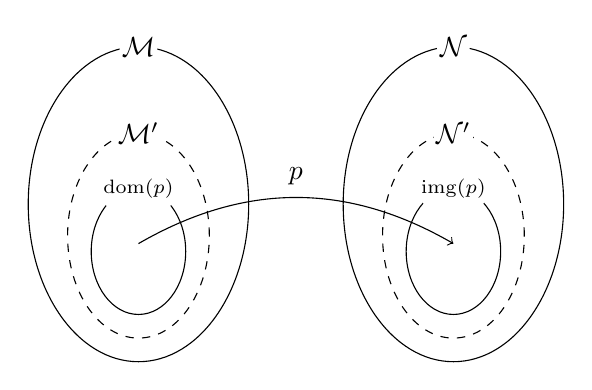
\begin{tikzpicture}
      \draw (-2,0) circle [x radius=1.4cm, y radius=2cm];
      \draw [dashed] (-2,-0.4) circle [x radius=0.9cm, y radius=1.3cm];
      \draw (-2,-0.6) circle [x radius=0.6cm, y radius=0.8cm];
      \draw (2,0) circle [x radius=1.4cm, y radius=2cm];
      \draw [dashed] (2,-0.4) circle [x radius=0.9cm, y radius=1.3cm];
      \draw (2,-0.6) circle [x radius=0.6cm, y radius=0.8cm];
      \node [fill=white, circle, inner sep=0] at (-2,2) {$\mathcal{M}$};
      \node [fill=white, circle, inner sep=0] at (-2,0.9) {$\mathcal{M}'$};
      \node [fill=white, circle, inner sep=0] at (-2,0.2) {$\scriptstyle\dom(p)$};
      \node [fill=white, circle, inner sep=0] at (2,2) {$\mathcal{N}$};
      \node [fill=white, circle, inner sep=0] at (2,0.9) {$\mathcal{N}'$};
      \node [fill=white, circle, inner sep=0] at (2,0.2) {$\scriptstyle\img(p)$};
      \draw [->] (-2,-0.5) to[bend left] (2,-0.5) node [pos=.5, label=above:$p$] {};
    \end{tikzpicture}
  \end{center}
  % picture
  Now $p$ is a \hyperlink{def:pe}{finite partial embedding} between countable models, so $p$ extends to an \hyperlink{def:iso}{isomorphism} $\pi: \mathcal{M}' \to \mathcal{N}'$ by \cref{thm:4.4}.
  In particular, $\pi$ is an \hyperlink{def:elmap}{elementary map} between $\mathcal{M}$ and $\mathcal{N}$.
\end{proof}
\begin{ncor}\label{cor:4.13}
  $(\mathbb{Q}, <) \preccurlyeq (\mathbb{R}, <)$.
\end{ncor}
\begin{proof}
  Use \cref{prop:4.12} with $\operatorname{id}: \mathbb{Q} \to \mathbb{R}$.
\end{proof}
\begin{ndef}[Random graph]\label{def:4.14}
  Let $L_{\text{gph}} = \{R\}$, a binary relation symbol.
  An $L_{\text{gph}}$-\hyperlink{def:lstr}{structure} is a \named{graph} if
  \begin{enumerate}[label=(\roman*)]
    \item $\forall x \; \lnot R(x,x)$
    \item $\forall xy \; (R(x,y) \leftrightarrow R(y,x))$
  \end{enumerate}

  \hypertarget{def:rgraph}An $L_{\text{gph}}$-\hyperlink{def:lstr}{structure} is a \named{random graph} if it is a graph such that, for all $n \in \omega$, axiom $(r_n)$ holds:
      \begin{equation*}
        \forall x_0 \dots x_n, y_0 \dots y_n \; \left(\bigwedge_{i,j=0}^n x_i \neq y_j \to \exists z \; \left(\bigwedge_{i=0}^n (z \neq x_i) \land (z \neq y_i) \land R(z,x_i) \land \lnot R(z, y_i)\right)\right)
      \end{equation*}
  \begin{enumerate}[label=(\roman*)]\setcounter{enumi}{2}
    \item $\exists xy \; (x \neq y)$.
  \end{enumerate}
\end{ndef}
Axiom $(r_n)$ effectively says that for disjoint subsets $(x_i)$ and $(y_i)$ each of size $n$, there is a (different) node $z$ connected to each $x_i$ and none of the $y_i$.
\begin{center}
  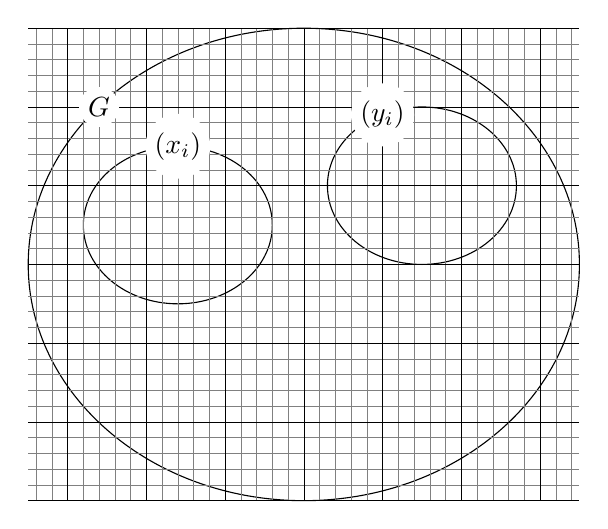
\begin{tikzpicture}
    \draw (0,0) circle [x radius=3.5cm, y radius=3cm];
    \draw (1.5,1) circle [x radius=1.2cm, y radius=1cm];
    \draw (-1.6,0.5) circle [x radius=1.2cm, y radius=1cm];
    \draw [help lines, step=0.2] (-3.5,-3) grid (3.5,3);
    \draw [help lines, black] (-3.5,-3) grid (3.5,3);
    \begin{scope}[every node/.style={fill=white, circle, inner sep=0.5mm}]
    \node at (-2.6,2) {$G$};
    \node at (-1.6, 1.5) {$(x_i)$};
    \node at (1, 1.9) {$(y_i)$};
    \end{scope}
  \end{tikzpicture}
\end{center}
\begin{remark}
  A \hyperlink{def:rgraph}{random graph} is infinite.
  Given a finite subset, we can always find a vertex that is connected to every vertex in the subset (likewise for not connected).
\end{remark}
\begin{nfact}\label{fact:4.15}
  There is a \hyperlink{def:rgraph}{random graph}.
\end{nfact}
\begin{proof}
  Let the domain be $\omega$, let $i,j \in \omega$ such that $i < j$.
  Write $j$ as a sum of distinct powers of $2$.
  Then $\{i,j\}$ is an edge iff $2^i$ appears in the sum.
\end{proof}
\begin{exercise}
  Prove that $\omega$ with this definition of $R$ is a \hyperlink{def:rgraph}{random graph}.
\end{exercise}
\begin{ndef}[Graph theories, partial embedding]\label{def:4.16}\hypertarget{def:gpe}
  $T_{\text{gph}}$ consists of the axioms (i),(ii) above, and $T_{\text{rg}} = T_{\text{gph}} \cup \{(\text{iii}), (r_n) : n \in \omega\}$.
  If $\mathcal{M}, \mathcal{N} \models T_{\text{gph}}$, a \index{partial embedding!graph}\textbf{partial embedding} is an injective map $p: A \subseteq M$ to $N$ such that
  \begin{equation*}
    \mathcal{M} \models R(a,b) \iff \mathcal{N} \models R(p(a), p(b))
  \end{equation*}
  for all $a,b$ in the domain.
  Just as before, if $|\dom(p)| < \omega$ then $p$ is called a \textbf{finite partial embedding}.
\end{ndef}
\begin{nlemma}\label{lem:4.17}
  Let $\mathcal{M} \models \hyperlink{def:gpe}{T_{\text{gph}}}$, $\mathcal{N} \models \hyperlink{def:gpe}{T_{\text{rg}}}$, let $p: A \subseteq M \to N$ be a \hyperlink{def:gpe}{finite partial embedding}, and let $c \in M$.
  Then there is $\hat{p}: \hat{A} \subseteq M \to N$ such that $\hat{p}$ is a partial embedding, $c \in \dom(\hat{p})$, $p \subseteq \hat{p}$.
\end{nlemma}

\begin{proof}
  \marginnote{\emph{Lecture 7}}[0cm]
  Take $c \in M$, $c \notin \dom(p)$.
  \begin{center}
    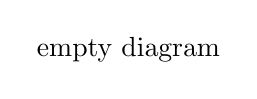
\begin{tikzpicture}
      \node {empty diagram};
    \end{tikzpicture}
  \end{center}
  Find $d \in N$ such that $N \models R(d, p(a)) \iff M \nModels R(c,a)$. %check this against notes
\end{proof}
\begin{nthm}\label{thm:4.18}
  Let $\mathcal{M}, \mathcal{N} \models \hyperlink{def:gpe}{T_{\text{rg}}}$ and $|\mathcal{M}| = |\mathcal{N}| = \omega$, and $p: A \subset M \to N$ is a \hyperlink{def:gpe}{finite partial embedding}.
  Then $\mathcal{M} \simeq \mathcal{N}$, by an isomorphism that extends $p$.
\end{nthm}
\begin{proof}
  Same as proof of \cref{thm:4.4}, but with \cref{lem:4.17} instead of \cref{lem:4.3}.
\end{proof}
\begin{ncor}
  \hyperlink{def:gpe}{$T_{\text{rg}}$} is \hyperlink{def:wcat}{$\omega$-categorical} and \hyperlink{def:complete}{complete}.
  Moreover, every \hyperlink{def:gpe}{finite partial embedding} between models of $T_{\text{rg}}$ is an \hyperlink{def:elmap}{elementary map}.
\end{ncor}
\begin{nremark}\label{rem:4.20}
  The unique (up to isomorphism) model of \hyperlink{def:gpe}{$T_{\text{rg}}$} is \emph{the} countable random graph, or the \named{Rado graph}.
  It is universal with respect to finite and countable graphs (i.e.\ it embeds them all).
  It is \named{ultrahomogeneous} i.e.\ every \hyperlink{def:iso}{isomorphism} between finite \hyperlink{def:subs}{substructures} extends to an automorphism of the whole graph.
\end{nremark}

\clearpage
\section{Compactness}
\begin{ndef}\label{def:5.1}
  Take an \hyperlink{def:ltheory}{$L$-theory} $T$.
  \begin{enumerate}[label=(\roman*)]
    \item \hypertarget{def:fs}$T$ is \named{finitely satisfiable} if every finite subset of \hyperlink{def:sentence}{sentences} in $T$ has a \hyperlink{def:model}{model}.
    \item \hypertarget{def:maximal}$T$ is \named{maximal} if for all $L$-sentences $\sigma$, either $\sigma \in T$ or $\lnot \sigma \in T$.
    \item \hypertarget{def:wp}$T$ has the \named{witness property} (WP) if for all $\phi(x)$ ($L$-\hyperlink{def:form}{formula} with one \hyperlink{def:free}{free} variable) there is a constant $c \in \mathscr{C}$ such that
      \begin{equation*}
        (\exists x \; \phi(x) \to \phi(c)) \in T.
      \end{equation*}
  \end{enumerate}
\end{ndef}
\begin{nlemma}\label{lem:5.2}
  If $T$ is \hyperlink{def:maximal}{maximal} and \hyperlink{def:fs}{finitely satisfiable} and $\phi$ is an $L$-\hyperlink{def:sentence}{sentence}, and $\Delta \overset{\mathclap{\text{finite}}}\subseteq T$ and $\Delta \hyperlink{def:models}{\models} \phi$, then $T \models \phi$.
\end{nlemma}
\begin{nlemma}\label{lem:5.3}
  Let $T$ be a \hyperlink{def:maximal}{maximal}, \hyperlink{def:fs}{finitely satisfiable} theory with the \hyperlink{def:wp}{witness property}. Then $T$ has a \hyperlink{def:model}{model}.
  Moreover, if $\lambda$ is a cardinal and $|\mathscr{C}| \leq \lambda$, then $T$ has a model of size at most $\lambda$.
\end{nlemma}
\begin{proof}
  Let $c,d \in \mathscr{C}$, define $c \sim d$ iff $c = d \in T$.

  \textbf{Claim:} $\sim$ is an equivalence relation. \textbf{Proof:} For transitivity, let $c \sim d$ and $d \sim e$.
  Then $c = d \in T$ and $d = e \in T$, so $c = e \in T$ (by \cref{lem:5.2}), and so $c \sim e$. $\blacksquare$

  \hypertarget{def:cstar}We denote $[c] \in \mathscr{C} / \sim$ by $c^*$

  Now, define a \hyperlink{def:lstr}{structure} $\mathcal{M}$ whose domain is $\mathscr{C} / \sim\ = M$.
  Clearly, $|M| \leq \lambda$ if $|\mathscr{C}| \leq \lambda$.
  We must define \hyperlink{def:lstr}{interpretations} in $\mathcal{M}$ for symbols of $L$.
  \begin{itemize}
    \item If $c \in \mathscr{C}$, then $c^\mathcal{M} = c^*$.
    \item If $R \in \mathscr{R}$, define
      \begin{equation*}
        R^\mathcal{M} \coloneqq \set{(c_1^*, \dotsc, c_{n_R}^*) | R(c_1, \dotsc, c_n) \in T}
      \end{equation*}
      \textbf{Claim:} $R^\mathcal{M}$ is well defined.
      \textbf{Proof:} Suppose $\bar{c}, \bar{d} \in \mathscr{C}^{n_R}$ and suppose $c_i \sim d_i$.
      That is, $c_i = d_i \in T$ for $i=1, \dotsc, n_R$
      \begin{equation*}
        R(\bar{c}) \in T \iff R(\bar{d}) \in T.
      \end{equation*}
      This proves that $R^\mathcal{M}$ is well defined. $\blacksquare$
    \item If $f \in \mathscr{F}$, and $\bar{c} \in \mathscr{C}^{n_R}$, then $f \bar{c} = d \in T$ for some $d \in \mathscr{C}$. (This is because $\exists x \; (f(\bar{c}) = x) \in T$ by \hyperlink{def:maximal}{maximality} and \hyperlink{def:fs}{finite satisfiability}.)

      Then define $f^\mathcal{M}(\bar{c}^*) = d^*$.
      Exercise: Check $f^\mathcal{M}(\bar{c}^*)$ is well-defined!
  \end{itemize}

  \textbf{Claim:} if $t(x_1, \dotsc, x_n)$ is an $L$-term and $c_1, \dotsc, c_n, d \in \mathscr{C}$, then
  \begin{equation*}
    t(c_1, \dotsc, c_n) = d \in T \iff t^\mathcal{M}(c_1^*, \dotsc, c_n^*) = d^*.
  \end{equation*}
  \textbf{Proof:}
  $(\Rightarrow)$ by induction on the complexity of $t$.
  $(\Leftarrow)$ Assume $t^\mathcal{M}(c_1^*, \dotsc, c_n^*) = d^*$.
  Then
  \begin{equation*}t(c_1, \dotsc, c_n) = e \in T\end{equation*}
  for some constant $e$.
  Use $\Rightarrow$ to get that $t^\mathcal{M}(c_1^*, \dotsc, c_n^*) = e^*$.
  But then $d^* = e^*$, i.e.\ $d = e \in T$.
  Then $t(c_1, \dotsc, c_n) = d \in T$. $\blacksquare$

  \textbf{Claim:} For all $L$-formulas $\phi(\bar{x})$, and $\bar{c} \in \mathscr{C}^{|\bar{x}|}$,
  \begin{equation*}
    \mathcal{M} \models \phi(\bar{c}) \iff \phi(\bar{c}) \in T.
  \end{equation*}
  \textbf{Proof:} By induction on $\phi(\bar{x})$. (Exercise: Fill in the details). $\blacksquare$
\end{proof}
\printindex
\end{document}
